\documentclass[twocolumn,a4paper,10pt]{article}
\usepackage[utf8]{inputenc}
\usepackage[T1]{fontenc}
\usepackage[english]{babel}
\usepackage{lmodern}
\usepackage[margin=1.8cm,top=2cm,bottom=1.8cm]{geometry}
\usepackage{amsmath}
\usepackage{booktabs}
\usepackage{graphicx}
\graphicspath{{figures/}}
\usepackage[font=small,skip=3pt]{caption}
\usepackage{tikz}
\usetikzlibrary{positioning, calc}
\usepackage{microtype}
\usepackage{titlesec}
\usepackage[colorlinks=true,linkcolor=black,citecolor=black,urlcolor=blue!50!black]{hyperref}

\setlength{\columnsep}{0.7cm}
\setlength{\parskip}{1pt}
\setlength{\textfloatsep}{8pt}
\setlength{\dbltextfloatsep}{9pt}
\titlespacing*{\section}{0pt}{6pt}{3pt}
\titleformat{\section}{\normalfont\large\bfseries}{\thesection}{0.6em}{}

\title{\vspace{-1.2cm}\Large\textbf{Portuguese Speech Synthesis with Tacotron2-VAE:\\ Style Copied from a Reference Recording}}
\author{\normalsize Beatriz Nunes \quad Herivelton Siqueira \quad Richard Viana\\[2pt]
\small Machine Learning II --- IMPA Tech\\
\small Instructors: Francisco Ganacim and Daniel Silveira Yukimura Lopez}
\date{\small Revised version --- November 2026}

\begin{document}

\twocolumn[
\maketitle
\vspace{-0.9cm}
\begin{center}
\begin{minipage}{0.92\textwidth}
\small\textbf{Abstract ---} We implement a speech synthesis system based on Tacotron~2 with a \textit{Variational Autoencoder} (VAE) that summarizes a reference recording into a style vector. This version replaces the previous one, whose central result (``interpretable spectral attention'') came from a code bug and was not valid. We fixed the bug, switched to training from a pretrained Tacotron~2, and checked every generated audio clip with speech recognition. The word error rate fell from 68\% to 2.2\% in English and from unintelligible to 10.5\% in Portuguese. With the VERBO emotional corpus, the generated speech copies the voice and pitch of the reference, at the cost of intelligibility; a style-strength control recovers intelligibility (9\% error) while keeping part of the emotion. Project page: \url{https://rick0110.github.io/ml2_final_project}.
\end{minipage}
\end{center}
\vspace{0.3cm}
]

\section{Introduction}
Speech synthesis systems produce intelligible speech, but with fixed intonation. Tacotron2-VAE \cite{hsu,zhang} compresses a \textbf{reference recording} into a latent vector $z$ that holds what the text does not determine (pitch, speed, voice) and conditions the synthesis: the text says what to say, the reference says how. Our goal is to have this system working in Portuguese, as the first piece of a dubbing system.

\section{Review of the previous version}
The previous version of this report proposed attention-based \textit{pooling} in the \textit{reference encoder} and interpreted its weights as bands of the spectrum. A review of the code revealed three problems. (i)~The mel of shape $(B, 80, T)$ was reshaped with \texttt{view} without transposing the axes: time and frequency were mixed up, and the position of the blocks changed with the batch \textit{padding}. The ``bands'' were an effect of this bug. (ii)~The comparison with the \textit{baseline} used runs of 11.2 thousand and 35.5 thousand iterations, and did not support the conclusion about latent collapse. (iii)~The audio was barely intelligible: transcribed by Whisper \cite{whisper}, the 26 English clips had on average 68\% of their words wrong, and the two Portuguese ones were not recognized. An extra \texttt{LayerNorm} in the decoder attention also prevented the use of pretrained weights. All results below are from the corrected version.

\section{Architecture}
The system (Fig.~\ref{fig:pipeline}) follows Tacotron~2 \cite{shen,nvidiataco}: a text \textit{encoder} (embedding + 3 Conv1d + BiLSTM), a location-sensitive attention, an autoregressive decoder that predicts the mel frame by frame together with the stop signal, and the universal \textbf{HiFi-GAN} vocoder \cite{hifigan}, pretrained and frozen. English enters as characters and Portuguese as IPA phonemes; both sets share the same table of 199 symbols, which makes it possible to adapt a model trained in English to Portuguese.

The \textit{reference encoder} \cite{skerry} applies 6 2D convolutions with \textit{stride}~2 to the reference mel and a GRU over the resulting $T/64$ time blocks ($\sim$0.74\,s each). The states $h_t$ are summarized by attention, $e=\sum_t \alpha_t h_t$ with $\alpha=\mathrm{softmax}(w^\top h_t+b)$, with zero weight on the \textit{padding} blocks. The summary is projected to $(\mu,\sigma)$; a 32-dimensional $z$ is sampled and converted into a style vector added to every position of the \textit{encoder} output. We did not compare this summary with the last GRU state, and therefore do not claim that it is better.

\begin{figure*}[t]
    \centering
    \resizebox{0.88\textwidth}{!}{%
    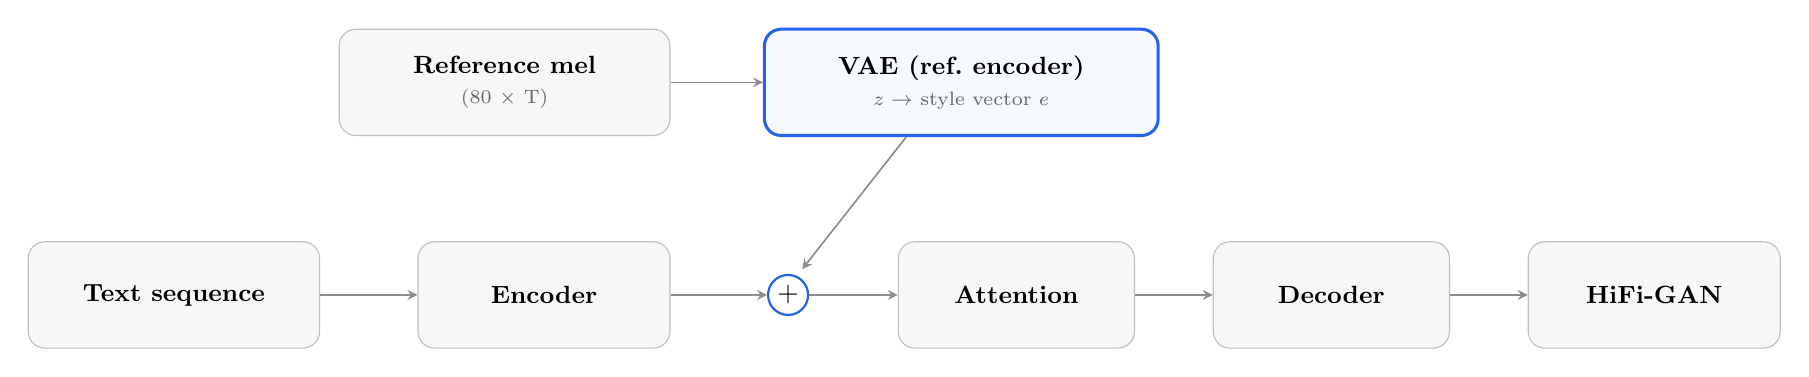
\begin{tikzpicture}[
        box/.style={rectangle, draw=black!25, rounded corners=6pt, fill=black!3, minimum height=1.35cm, text centered, font=\small\bfseries, align=center, inner xsep=10pt},
        boxhl/.style={box, draw=refblue, line width=1.1pt, fill=refblue!4},
        arrow/.style={->, >=stealth, semithick, draw=black!45}
    ]
    \definecolor{refblue}{RGB}{37,99,235}
    % top row (style branch)
    \node[box, minimum width=4.2cm] (mel) at (6.6,0) {Reference mel\\{\scriptsize\mdseries\color{black!60}(80 $\times$ T)}};
    \node[boxhl, minimum width=5cm] (vae) at (12.4,0) {VAE (ref.\ encoder)\\{\scriptsize\mdseries\color{black!60}$z \rightarrow$ style vector $e$}};
    % bottom row (main pipeline)
    \node[box, minimum width=3.7cm] (texto) at (2.4,-2.7) {Text sequence};
    \node[box, minimum width=3.2cm] (encoder) at (7.1,-2.7) {Encoder};
    \node[circle, draw=refblue, thick, fill=white, inner sep=1.5pt, font=\normalsize] (soma) at (10.2,-2.7) {$+$};
    \node[box, minimum width=3cm] (atencao) at (13.1,-2.7) {Attention};
    \node[box, minimum width=3cm] (decoder) at (17.1,-2.7) {Decoder};
    \node[box, minimum width=3.2cm] (waveglow) at (21.2,-2.7) {HiFi-GAN};
    % arrows
    \draw[arrow] (mel) -- (vae);
    \draw[arrow] ([xshift=-0.7cm]vae.south) -- ($(soma.north)+(0.18,0.06)$);
    \draw[arrow] (texto) -- (encoder);
    \draw[arrow] (encoder) -- (soma);
    \draw[arrow] (soma) -- (atencao);
    \draw[arrow] (atencao) -- (decoder);
    \draw[arrow] (decoder) -- (waveglow);
    \end{tikzpicture}%
    }
    \caption{\small System architecture: the VAE compresses the reference mel into the style vector $e$, added ($+$) to every position of the \textit{encoder} memory; attention and decoder generate the mel spectrogram, converted into audio by HiFi-GAN.}
    \label{fig:pipeline}
\end{figure*}

\section{Training}
The loss combines four terms:
\begin{equation*}
\mathcal{L} = \mathcal{L}_{\text{mel}} + \mathcal{L}_{\text{gate}} + \beta(\text{step})\,\mathcal{L}_{\text{KL}} + \lambda\,\mathcal{L}_{\text{GA}},
\end{equation*}
with the mel MSE, the cross-entropy of the stop signal, the KL with \textit{free bits} of 0.5 and a cyclical $\beta$ (0 to 0.2), and guided attention \cite{tachibana}. Training from scratch did not fit the budget and was the likely cause of the poor alignments; training is therefore done in stages, each starting from the previous one (Tab.~\ref{tab:etapas}), on an L4 GPU, with Adam ($lr=10^{-4}$) and 28.9\,M parameters.

\begin{table}[h]
\centering\small
\begin{tabular}{@{}llr@{}}
\toprule
Stage & Data & Steps\\
\midrule
English & LJSpeech, 23.7\,h & 2,500\\
Portuguese & TTS-Portuguese \cite{ttspt}, 3.8\,h & 4,000\\
Emotion & TTS-Port. + VERBO \cite{verbo} & 1,500\\
\bottomrule
\end{tabular}
\caption{Training stages. The first starts from NVIDIA's pretrained Tacotron~2; each of the following starts from the previous one. VERBO has 1,167 utterances from 12 speakers in 7 emotions, with only 14 distinct sentences.}
\label{tab:etapas}
\end{table}

\begin{figure}[t]
    \centering
    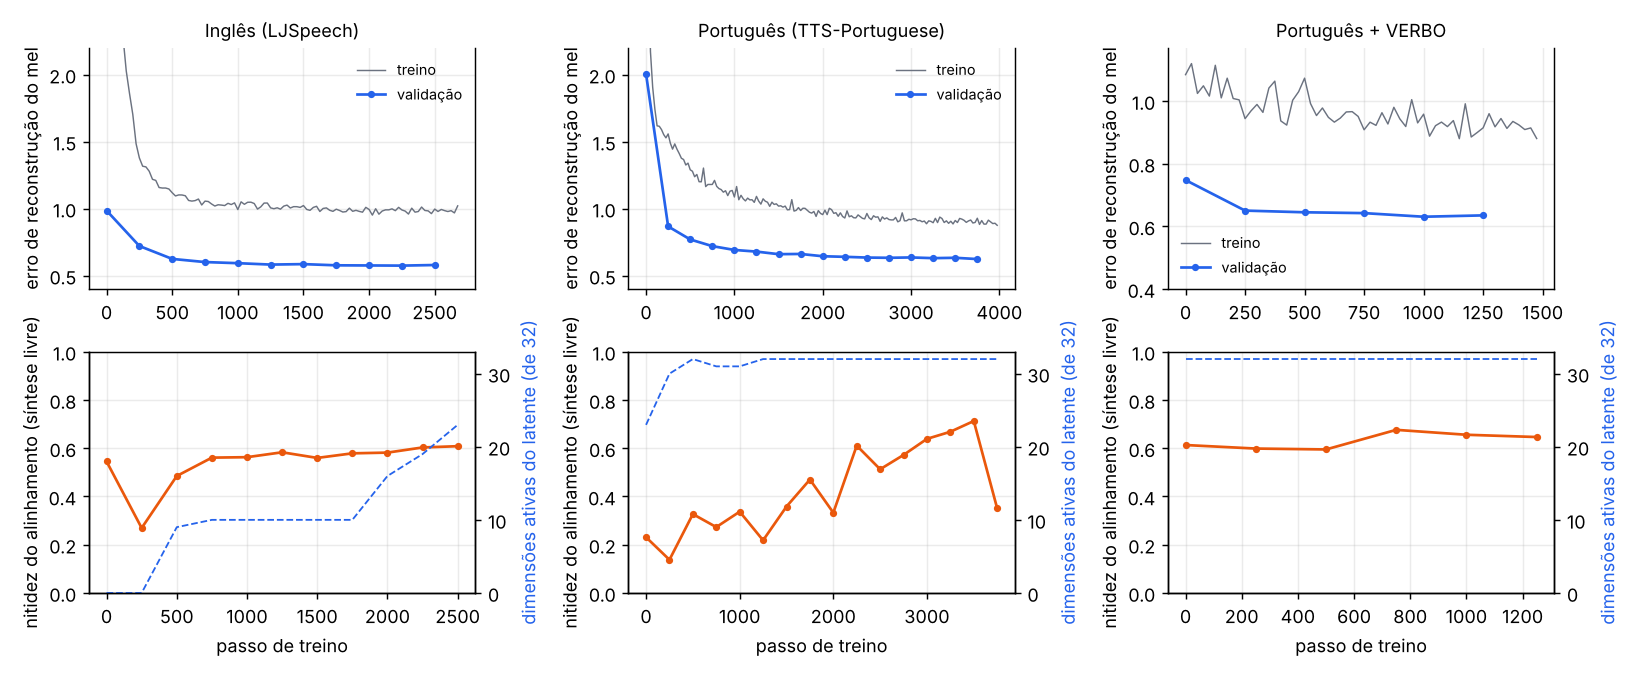
\includegraphics[width=\columnwidth]{fig_retraining_curves}
    \caption{Top: mel reconstruction error (training in gray, validation in blue; training is higher because half of the decoder input frames are dropped). Bottom: alignment sharpness in free-running synthesis (orange) and active latent dimensions (dashed).}
    \label{fig:curvas}
\end{figure}

\section{Evaluation}
For each model we synthesize 6 sentences outside the training set with several references. Each clip is transcribed by Whisper \textit{small} and compared with the requested text (word error rate, WER). We also measure whether the decoder stops on its own, the mean pitch (F0) and the speed (characters per second) of the generated audio and of the reference.

\begin{figure}[t]
    \centering
    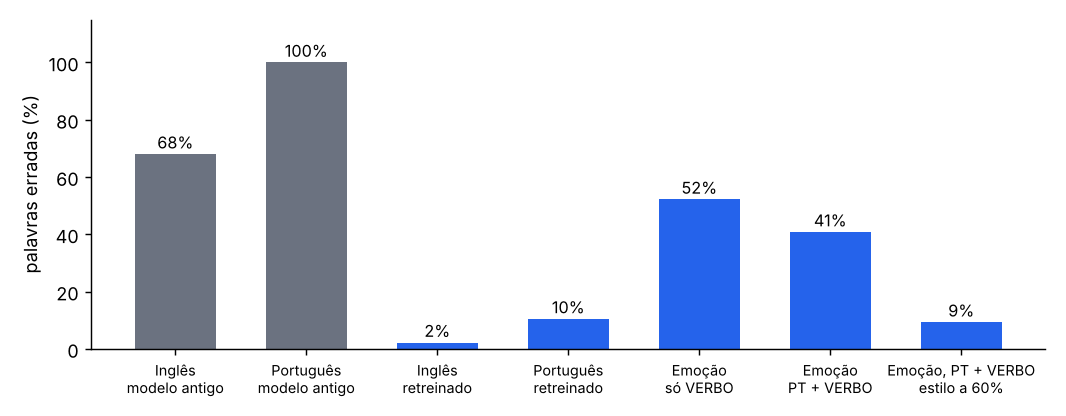
\includegraphics[width=\columnwidth]{fig_retraining_wer}
    \caption{Word errors in the automatic transcription of the generated audio. Gray: previous models. Blue: retrained.}
    \label{fig:wer}
\end{figure}

\textbf{English.} WER of 2.2\% over 18 clips, all stopping on their own; the three errors are the same word (``stone''). Pitch and speed did not follow the references: LJSpeech is a single female speaker with uniform reading, and there is little style variation to learn.

\textbf{Portuguese.} WER of 10.5\% over 18 clips, all stopping on their own (Fig.~\ref{fig:wer}). The errors are isolated substitutions (``carrega''$\to$``cariga''). Speaking speed follows the reference: with references of 9.1, 12.6 and 16.3 characters/s, the same sentence came out at 8.8, 11.9 and 12.7. All 32 latent dimensions remain active (Fig.~\ref{fig:curvas}).

\begin{figure}[t]
    \centering
    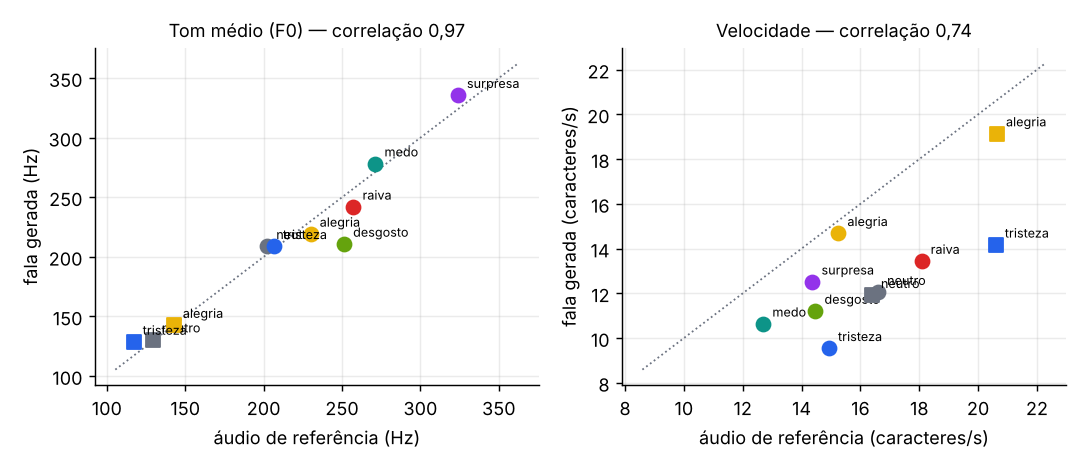
\includegraphics[width=\columnwidth]{fig_retraining_style_ptverbo_vae_v1}
    \caption{Portuguese + VERBO model, full style: pitch and speed of the generated speech against those of the reference (circles: female speaker f1; squares: male speaker m1).}
    \label{fig:estilo}
\end{figure}

\begin{figure}[t]
    \centering
    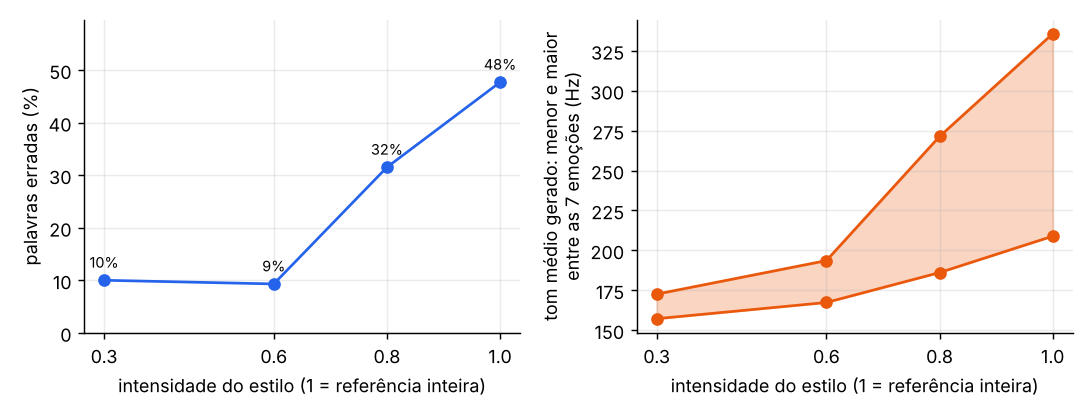
\includegraphics[width=\columnwidth]{fig_retraining_strength}
    \caption{Effect of style strength (7 emotions of female speaker f1): word errors and range of mean pitch across emotions.}
    \label{fig:intensidade}
\end{figure}

\textbf{Emotion.} We use 10 VERBO references (7 emotions of female speaker f1 and 3 of male speaker m1). The Portuguese model, without having seen VERBO, keeps its own voice (WER 19\%, with no relation between the generated pitch and that of the reference). Fine-tuned on VERBO alone, the model copies voice and pitch (correlation of 0.96 between the generated F0 and that of the reference), but WER rises to 52\%: with 14 sentences, it unlearns how to read new text. Training on both corpora together, pitch still follows the reference (correlation 0.97, Fig.~\ref{fig:estilo}) and WER drops to 41\%, still high.

\textbf{Style strength.} The error comes from synthesizing with voices the model has heard in only 14 sentences. Multiplying the latent code of the reference by a factor $a\in[0,1]$ before synthesis, $z = a\,\mu_{\text{ref}}$, we obtain a continuous control (Fig.~\ref{fig:intensidade}): with $a=0.6$ WER drops to 9\% and speed still varies with the emotion (from 9.3 to 14.1 characters/s), but pitch stays close to neutral. Strong emotion and clear speech were not obtained at the same time; the limit lies in the corpus, not in the model.

\section{Data coverage and style}
The previous section attributes the error with strong emotion to the corpus: the style appears in few sentences. We test this in a controlled way, with voices in place of emotions. Training combines 2,000 LJSpeech sentences (default voice, with plenty of text) with $N$ LibriTTS speakers with $K$ sentences each, starting from the English model, for 2,500 steps. We synthesize 25 sentences outside the training set with 8 references from trained voices and 4 from never-seen voices. A voice counts as copied when the generated audio is more similar to the reference than to the default voice, according to an external speaker encoder (Resemblyzer).

\begin{figure}[t]
    \centering
    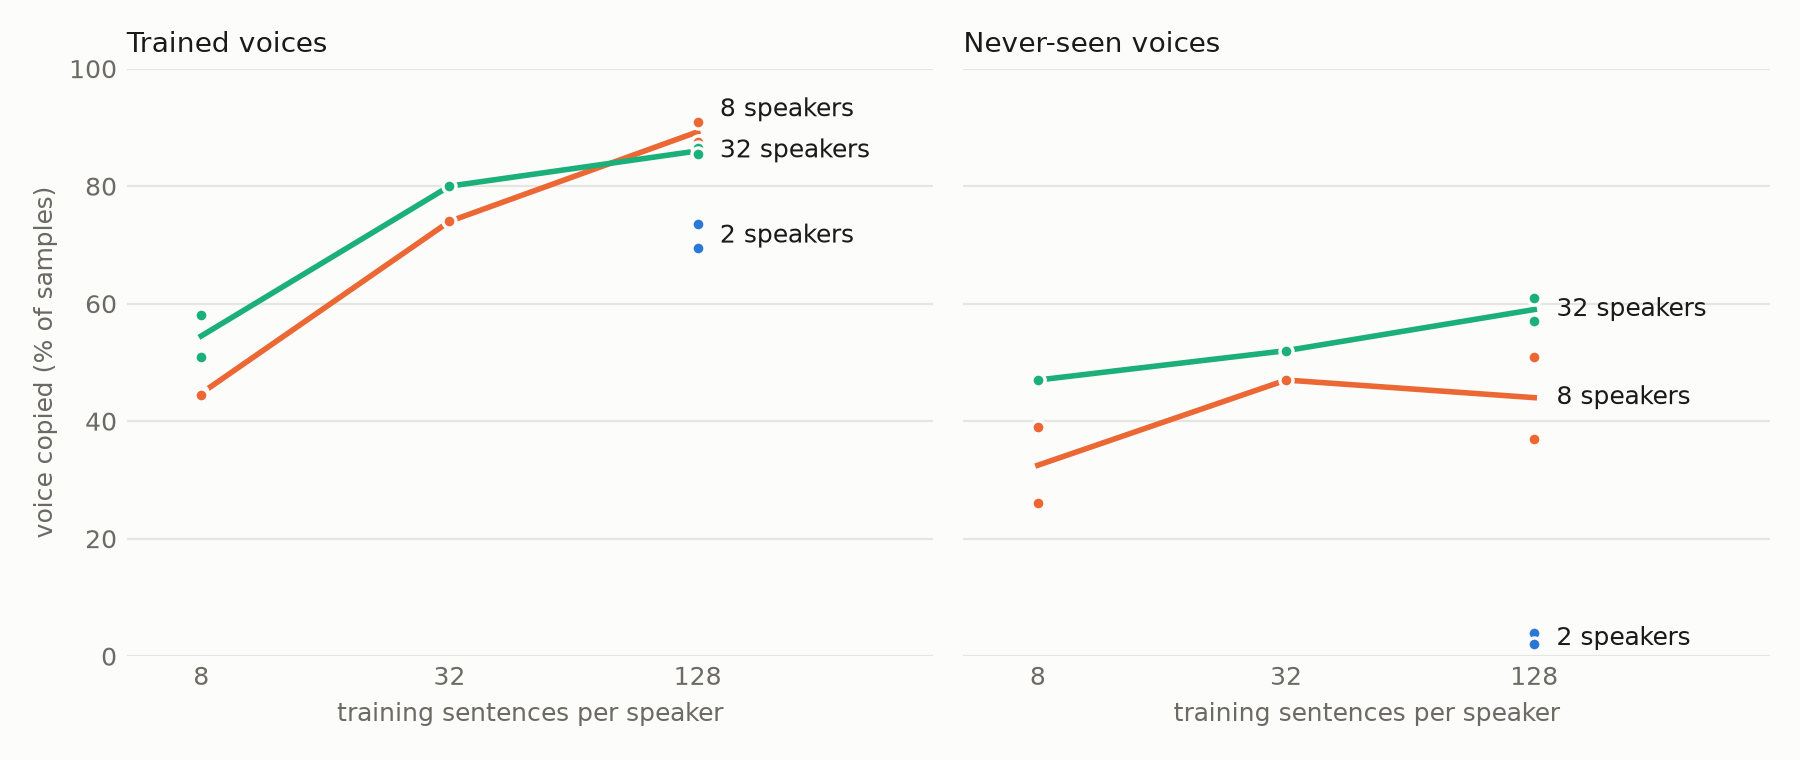
\includegraphics[width=\columnwidth]{fig_coverage}
    \caption{Share of samples with the voice copied, by sentences per speaker ($K$) and number of speakers ($N$). Points: seeds; lines: means.}
    \label{fig:cobertura}
\end{figure}

\begin{table}[t]
\centering\footnotesize
\begin{tabular}{rrcccc}
\toprule
 & & \multicolumn{2}{c}{WER (\%)} & \multicolumn{2}{c}{Voice copied (\%)} \\
$N$ & $K$ & trained & new & trained & new \\
\midrule
2 & 128 & 13 / 11 & 8 / 5 & 70 / 74 & 4 / 2 \\
8 & 8 & 21 / 26 & 14 / 24 & 45 / 44 & 26 / 39 \\
8 & 32 & 17 & 14 & 74 & 47 \\
8 & 128 & 11 / 10 & 8 / 9 & 91 / 88 & 51 / 37 \\
32 & 8 & 17 / 17 & 13 / 9 & 58 / 51 & 47 / 47 \\
32 & 32 & 13 & 8 & 80 & 52 \\
32 & 128 & 12 / 10 & 5 / 5 & 86 / 86 & 61 / 57 \\
\bottomrule
\end{tabular}
\caption{Coverage experiment (full style). Two values: two seeds.}
\label{tab:cobertura}
\end{table}

The two factors play different roles (Fig.~\ref{fig:cobertura}, Tab.~\ref{tab:cobertura}). The number of sentences per speaker decides whether trained voices are copied: with 8 speakers, 45\%, 74\% and 90\% for $K=8$, 32 and 128. The number of speakers decides whether new voices are copied: with $K=128$, 3\%, 44\% and 59\% for $N=2$, 8 and 32. With 32 speakers and only 8 sentences each, new voices are copied as well as with 8 speakers and 128 sentences. The latent space explains the trade-off with intelligibility: over 144 references, the distance from the style code to the center of the default voice has a rank correlation of 0.83 with voice copying and 0.45 with WER, and about 80\% of the latent variance is difference between speakers. A direct test of the hypothesis that the style code carries the sentence content gave a negative result: taking the style from another sentence of the same speaker during training, copying of trained voices stood at 52\% and 48\% (versus 45\% and 44\%) and that of new voices at 27\% and 32\% (versus 26\% and 39\%) with $N=8$, $K=8$, and at 87\% and 38\% (versus 91\% and 51\%) with $K=128$, all within the variation between seeds. Adding a contrastive loss on the latent (same speaker as the positive pair, other speakers as negatives) did not change the picture either: 42\% and 48\% of trained voices and 27\% and 31\% of new ones with $K=8$, 85\% and 39\% with $K=128$. The bottleneck appears to be the coverage of voices and sentences seen by the decoder, not the sentence content in the latent. A second style input, the vector of a pretrained, frozen speaker encoder (ECAPA-TDNN) added to the encoded text, is ignored by training: with the VAE zeroed, no voice is copied (0\% in three runs). Zeroing the VAE vector in half of the training items, the speaker vector starts being used, but on its own it copies 71\% of trained voices and 5\% of new ones with $N=8$, $K=128$, and 64\% and 47\% with $N=32$, $K=128$; together with the VAE, 62\% of new voices, the same as normal training (61\% and 57\%). The limit is the number of voices the decoder has heard, whatever path the voice takes to reach it. Creating pseudo-speakers by changing the speed of the recordings (each training sentence gains a copy 1.5 to 4 semitones higher or lower) does not help either: 28\% and 42\% of new voices copied with $N=8$ and $K=8$ and 128, within the range of normal training; a law $a + A/N + B/(NK)$ fitted to the 12 runs predicted 31\% and 44\% for this case (\texttt{reports/theory/coverage\_theory.md}). What counts is the number of real voices. With 128 speakers, the same law got the $K=8$ run right (55\% of new voices copied, predicted 56\%) and overshot with $K=32$ (74\%, predicted 57\%); the replica with another seed gave 56\% (mean 65\%) and 200 speakers gave 64\%, which looked like a ceiling. Evaluated on 38 voices from another subset (950 samples per run), however, the $K=32$ runs copy 57\%, 70\% and 79\% of the voices for $N=8$, 32 and 128, with a WER of 12--13\%: the gain from 32 to 128 speakers (9 points, 95\% CI from 1.5 to 17) is almost that from 8 to 32; the shape of the curve is not yet identifiable with three points. Limitations: several configurations have only one seed, each run evaluates 4 new voices, and copying of new voices varies by up to 18 points between seeds.

\section{Conclusion}
The central result of the previous version was a bug and has been withdrawn. With the corrected code and training from a pretrained model, the system speaks English and Portuguese intelligibly and copies the speed from the reference and, with data from several speakers and emotions, the voice and pitch. With VERBO, copying the emotion in full costs intelligibility, and the style-strength control makes it possible to choose the operating point of this trade-off. Limitations: the evaluation uses few sentences and measures only intelligibility, not naturalness; the style vector is global and does not vary along the sentence; attention \textit{pooling} was not compared with the simpler alternative. For dubbing, duration control of the utterances, video as input, and lip sync are still missing.

\begin{thebibliography}{99}\footnotesize\setlength{\itemsep}{1pt}\setlength{\parskip}{0pt}
\bibitem{hsu} Hsu, W.-N. et al. \textit{Hierarchical Generative Modeling for Controllable Speech Synthesis}. ICLR, 2019.
\bibitem{zhang} Zhang, Y.-J., Pan, S., He, L., Ling, Z.-H. \textit{Learning Latent Representations for Style Control and Transfer in End-to-End Speech Synthesis}. ICASSP, 2019. arXiv:1812.04342.
\bibitem{shen} Shen, J. et al. \textit{Natural TTS Synthesis by Conditioning WaveNet on Mel Spectrogram Predictions}. ICASSP, 2018. arXiv:1712.05884.
\bibitem{nvidiataco} NVIDIA. \textit{Tacotron 2} (reference implementation). \url{https://github.com/NVIDIA/tacotron2}.
\bibitem{hifigan} Kong, J., Kim, J., Bae, J. \textit{HiFi-GAN: Generative Adversarial Networks for Efficient and High Fidelity Speech Synthesis}. NeurIPS, 2020.
\bibitem{skerry} Skerry-Ryan, R.J. et al. \textit{Towards End-to-End Prosody Transfer for Expressive Speech Synthesis with Tacotron}. ICML, 2018.
\bibitem{tachibana} Tachibana, H. et al. \textit{Efficiently Trainable Text-to-Speech System Based on Deep Convolutional Networks with Guided Attention}. 2017.
\bibitem{ttspt} Casanova, E. et al. \textit{TTS-Portuguese Corpus: a corpus for speech synthesis in Brazilian Portuguese}. Language Resources and Evaluation, 2022.
\bibitem{verbo} Torres Neto, J. R. et al. \textit{VERBO: Voice Emotion Recognition dataBase in Portuguese Language}. Journal of Computer Science, 2018.
\bibitem{whisper} Radford, A. et al. \textit{Robust Speech Recognition via Large-Scale Weak Supervision}. ICML, 2023.
\end{thebibliography}

\end{document}
